\documentclass[1p]{elsarticle_modified}
%\bibliographystyle{elsarticle-num}

%\usepackage[colorlinks]{hyperref}
%\usepackage{abbrmath_seonhwa} %\Abb, \Ascr, \Acal ,\Abf, \Afrak
\usepackage{amsfonts}
\usepackage{amssymb}
\usepackage{amsmath}
\usepackage{amsthm}
\usepackage{scalefnt}
\usepackage{amsbsy}
\usepackage{kotex}
\usepackage{caption}
\usepackage{subfig}
\usepackage{color}
\usepackage{graphicx}
\usepackage{xcolor} %% white, black, red, green, blue, cyan, magenta, yellow
\usepackage{float}
\usepackage{setspace}
\usepackage{hyperref}

\usepackage{tikz}
\usetikzlibrary{arrows}

\usepackage{multirow}
\usepackage{array} % fixed length table
\usepackage{hhline}

%%%%%%%%%%%%%%%%%%%%%
\makeatletter
\renewcommand*\env@matrix[1][\arraystretch]{%
	\edef\arraystretch{#1}%
	\hskip -\arraycolsep
	\let\@ifnextchar\new@ifnextchar
	\array{*\c@MaxMatrixCols c}}
\makeatother %https://tex.stackexchange.com/questions/14071/how-can-i-increase-the-line-spacing-in-a-matrix
%%%%%%%%%%%%%%%

\usepackage[normalem]{ulem}

\newcommand{\msout}[1]{\ifmmode\text{\sout{\ensuremath{#1}}}\else\sout{#1}\fi}
%SOURCE: \msout is \stkout macro in https://tex.stackexchange.com/questions/20609/strikeout-in-math-mode

\newcommand{\cancel}[1]{
	\ifmmode
	{\color{red}\msout{#1}}
	\else
	{\color{red}\sout{#1}}
	\fi
}

\newcommand{\add}[1]{
	{\color{blue}\uwave{#1}}
}

\newcommand{\replace}[2]{
	\ifmmode
	{\color{red}\msout{#1}}{\color{blue}\uwave{#2}}
	\else
	{\color{red}\sout{#1}}{\color{blue}\uwave{#2}}
	\fi
}

\newcommand{\Sol}{\mathcal{S}} %segment
\newcommand{\D}{D} %diagram
\newcommand{\A}{\mathcal{A}} %arc


%%%%%%%%%%%%%%%%%%%%%%%%%%%%%5 test

\def\sl{\operatorname{\textup{SL}}(2,\Cbb)}
\def\psl{\operatorname{\textup{PSL}}(2,\Cbb)}
\def\quan{\mkern 1mu \triangleright \mkern 1mu}

\theoremstyle{definition}
\newtheorem{thm}{Theorem}[section]
\newtheorem{prop}[thm]{Proposition}
\newtheorem{lem}[thm]{Lemma}
\newtheorem{ques}[thm]{Question}
\newtheorem{cor}[thm]{Corollary}
\newtheorem{defn}[thm]{Definition}
\newtheorem{exam}[thm]{Example}
\newtheorem{rmk}[thm]{Remark}
\newtheorem{alg}[thm]{Algorithm}

\newcommand{\I}{\sqrt{-1}}
\begin{document}

%\begin{frontmatter}
%
%\title{Boundary parabolic representations of knots up to 8 crossings}
%
%%% Group authors per affiliation:
%\author{Yunhi Cho} 
%\address{Department of Mathematics, University of Seoul, Seoul, Korea}
%\ead{yhcho@uos.ac.kr}
%
%
%\author{Seonhwa Kim} %\fnref{s_kim}}
%\address{Center for Geometry and Physics, Institute for Basic Science, Pohang, 37673, Korea}
%\ead{ryeona17@ibs.re.kr}
%
%\author{Hyuk Kim}
%\address{Department of Mathematical Sciences, Seoul National University, Seoul 08826, Korea}
%\ead{hyukkim@snu.ac.kr}
%
%\author{Seokbeom Yoon}
%\address{Department of Mathematical Sciences, Seoul National University, Seoul, 08826,  Korea}
%\ead{sbyoon15@snu.ac.kr}
%
%\begin{abstract}
%We find all boundary parabolic representation of knots up to 8 crossings.
%
%\end{abstract}
%\begin{keyword}
%    \MSC[2010] 57M25 
%\end{keyword}
%
%\end{frontmatter}

%\linenumbers
%\tableofcontents
%
\newcommand\colored[1]{\textcolor{white}{\rule[-0.35ex]{0.8em}{1.4ex}}\kern-0.8em\color{red} #1}%
%\newcommand\colored[1]{\textcolor{white}{ #1}\kern-2.17ex	\textcolor{white}{ #1}\kern-1.81ex	\textcolor{white}{ #1}\kern-2.15ex\color{red}#1	}

{\Large $\underline{11a_{340}~(K11a_{340})}$}

\setlength{\tabcolsep}{10pt}
\renewcommand{\arraystretch}{1.6}
\vspace{1cm}\begin{tabular}{m{100pt}>{\centering\arraybackslash}m{274pt}}
\multirow{5}{120pt}{
	\centering
	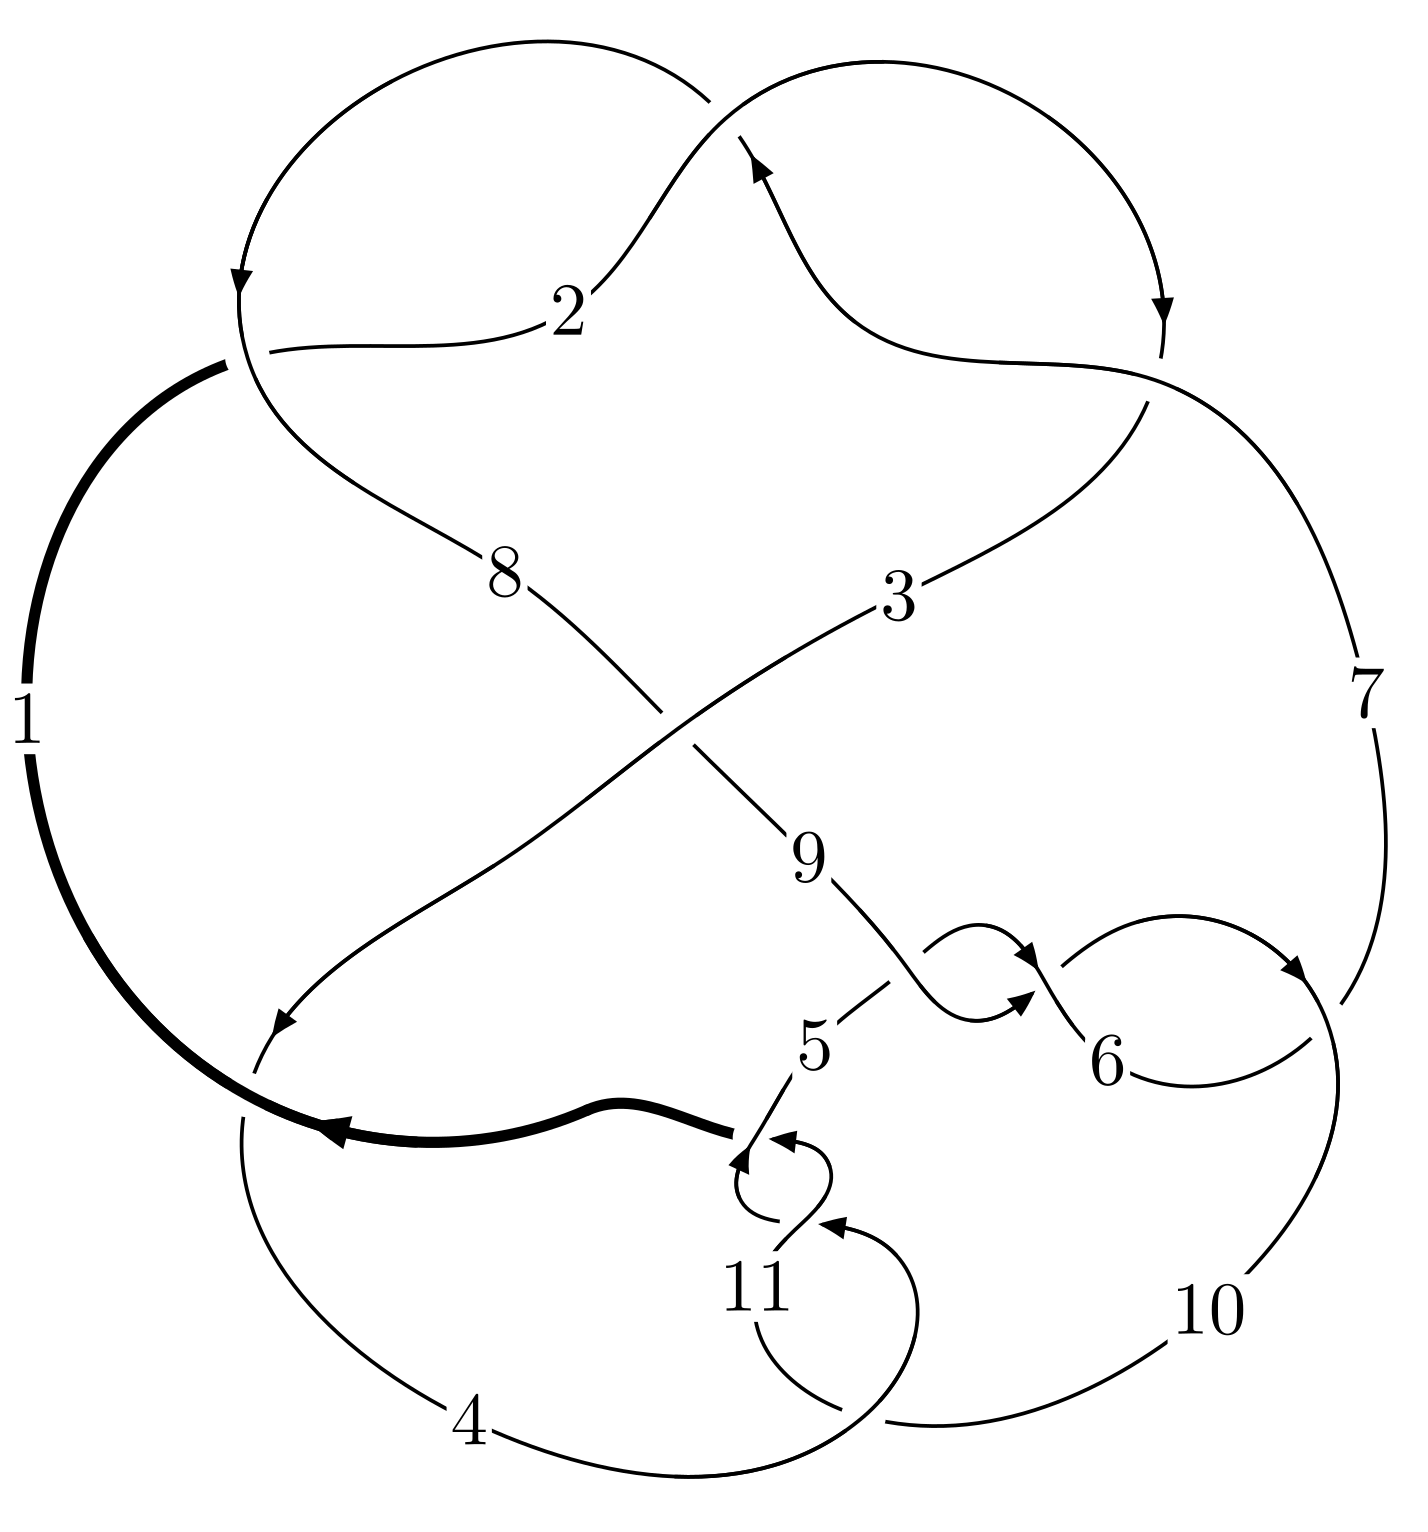
\includegraphics[width=112pt]{../../../GIT/diagram.site/Diagrams/png/589_11a_340.png}\\
\ \ \ A knot diagram\footnotemark}&
\allowdisplaybreaks
\textbf{Linearized knot diagam} \\
\cline{2-2}
 &
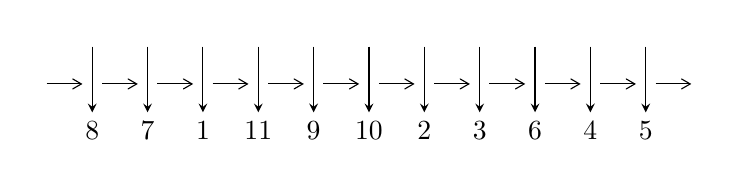
\begin{tikzpicture}[x=20pt, y=17pt]
	% nodes
	\node (C0) at (0, 0) {};
	\node (C1) at (1, 0) {};
	\node (C1U) at (1, +1) {};
	\node (C1D) at (1, -1) {8};

	\node (C2) at (2, 0) {};
	\node (C2U) at (2, +1) {};
	\node (C2D) at (2, -1) {7};

	\node (C3) at (3, 0) {};
	\node (C3U) at (3, +1) {};
	\node (C3D) at (3, -1) {1};

	\node (C4) at (4, 0) {};
	\node (C4U) at (4, +1) {};
	\node (C4D) at (4, -1) {11};

	\node (C5) at (5, 0) {};
	\node (C5U) at (5, +1) {};
	\node (C5D) at (5, -1) {9};

	\node (C6) at (6, 0) {};
	\node (C6U) at (6, +1) {};
	\node (C6D) at (6, -1) {10};

	\node (C7) at (7, 0) {};
	\node (C7U) at (7, +1) {};
	\node (C7D) at (7, -1) {2};

	\node (C8) at (8, 0) {};
	\node (C8U) at (8, +1) {};
	\node (C8D) at (8, -1) {3};

	\node (C9) at (9, 0) {};
	\node (C9U) at (9, +1) {};
	\node (C9D) at (9, -1) {6};

	\node (C10) at (10, 0) {};
	\node (C10U) at (10, +1) {};
	\node (C10D) at (10, -1) {4};

	\node (C11) at (11, 0) {};
	\node (C11U) at (11, +1) {};
	\node (C11D) at (11, -1) {5};
	\node (C12) at (12, 0) {};

	% arrows
	\draw[->,>={angle 60}]
	(C0) edge (C1) (C1) edge (C2) (C2) edge (C3) (C3) edge (C4) (C4) edge (C5) (C5) edge (C6) (C6) edge (C7) (C7) edge (C8) (C8) edge (C9) (C9) edge (C10) (C10) edge (C11) (C11) edge (C12) ;	\draw[->,>=stealth]
	(C1U) edge (C1D) (C2U) edge (C2D) (C3U) edge (C3D) (C4U) edge (C4D) (C5U) edge (C5D) (C6U) edge (C6D) (C7U) edge (C7D) (C8U) edge (C8D) (C9U) edge (C9D) (C10U) edge (C10D) (C11U) edge (C11D) ;
	\end{tikzpicture} \\
\hhline{~~} \\& 
\textbf{Solving Sequence} \\ \cline{2-2} 
 &
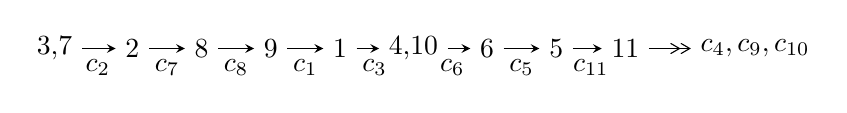
\begin{tikzpicture}[x=25pt, y=7pt]
	% node
	\node (A0) at (-1/8, 0) {3,7};
	\node (A1) at (1, 0) {2};
	\node (A2) at (2, 0) {8};
	\node (A3) at (3, 0) {9};
	\node (A4) at (4, 0) {1};
	\node (A5) at (81/16, 0) {4,10};
	\node (A6) at (49/8, 0) {6};
	\node (A7) at (57/8, 0) {5};
	\node (A8) at (65/8, 0) {11};
	\node (C1) at (1/2, -1) {$c_{2}$};
	\node (C2) at (3/2, -1) {$c_{7}$};
	\node (C3) at (5/2, -1) {$c_{8}$};
	\node (C4) at (7/2, -1) {$c_{1}$};
	\node (C5) at (9/2, -1) {$c_{3}$};
	\node (C6) at (45/8, -1) {$c_{6}$};
	\node (C7) at (53/8, -1) {$c_{5}$};
	\node (C8) at (61/8, -1) {$c_{11}$};
	\node (A9) at (10, 0) {$c_{4},c_{9},c_{10}$};

	% edge
	\draw[->,>=stealth]	
	(A0) edge (A1) (A1) edge (A2) (A2) edge (A3) (A3) edge (A4) (A4) edge (A5) (A5) edge (A6) (A6) edge (A7) (A7) edge (A8) ;
	\draw[->>,>={angle 60}]	
	(A8) edge (A9);
\end{tikzpicture} \\ 

\end{tabular} \\

\footnotetext{
The image of knot diagram is generated by the software ``\textbf{Draw programme}" developed by Andrew Bartholomew(\url{http://www.layer8.co.uk/maths/draw/index.htm\#Running-draw}), where we modified some parts for our purpose(\url{https://github.com/CATsTAILs/LinksPainter}).
}\phantom \\ \newline 
\centering \textbf{Ideals for irreducible components\footnotemark of $X_{\text{par}}$} 
 
\begin{align*}
I^u_{1}&=\langle 
- u^{16}+2 u^{15}+\cdots+b-1,\;u^{17}- u^{16}+\cdots+2 a+6 u,\;u^{18}-3 u^{17}+\cdots-4 u+2\rangle \\
I^u_{2}&=\langle 
u^{12} a+u^{11} a+\cdots+b+a,\;u^{12}+u^{11}+\cdots+a^2- a,\\
\phantom{I^u_{2}}&\phantom{= \langle  }u^{14}+u^{13}+7 u^{12}+6 u^{11}+18 u^{10}+13 u^9+19 u^8+10 u^7+4 u^6-2 u^5-4 u^4-4 u^3+u+1\rangle \\
I^u_{3}&=\langle 
b-1,\;2 a+u,\;u^2+2\rangle \\
\\
I^v_{1}&=\langle 
a,\;b+1,\;v+1\rangle \\
\end{align*}
\raggedright * 4 irreducible components of $\dim_{\mathbb{C}}=0$, with total 49 representations.\\
\footnotetext{All coefficients of polynomials are rational numbers. But the coefficients are sometimes approximated in decimal forms when there is not enough margin.}
\newpage
\renewcommand{\arraystretch}{1}
\centering \section*{I. $I^u_{1}= \langle - u^{16}+2 u^{15}+\cdots+b-1,\;u^{17}- u^{16}+\cdots+2 a+6 u,\;u^{18}-3 u^{17}+\cdots-4 u+2 \rangle$}
\flushleft \textbf{(i) Arc colorings}\\
\begin{tabular}{m{7pt} m{180pt} m{7pt} m{180pt} }
\flushright $a_{3}=$&$\begin{pmatrix}1\\0\end{pmatrix}$ \\
\flushright $a_{7}=$&$\begin{pmatrix}0\\u\end{pmatrix}$ \\
\flushright $a_{2}=$&$\begin{pmatrix}1\\- u^2\end{pmatrix}$ \\
\flushright $a_{8}=$&$\begin{pmatrix}- u\\u^3+u\end{pmatrix}$ \\
\flushright $a_{9}=$&$\begin{pmatrix}- u^3-2 u\\u^3+u\end{pmatrix}$ \\
\flushright $a_{1}=$&$\begin{pmatrix}u^2+1\\- u^4-2 u^2\end{pmatrix}$ \\
\flushright $a_{4}=$&$\begin{pmatrix}- u^6-3 u^4-2 u^2+1\\u^8+4 u^6+4 u^4\end{pmatrix}$ \\
\flushright $a_{10}=$&$\begin{pmatrix}-\frac{1}{2} u^{17}+\frac{1}{2} u^{16}+\cdots+u^2-3 u\\u^{16}-2 u^{15}+\cdots-3 u^2+1\end{pmatrix}$ \\
\flushright $a_{6}=$&$\begin{pmatrix}\frac{1}{2} u^{17}-\frac{3}{2} u^{16}+\cdots+2 u-2\\u^{14}- u^{13}+\cdots+u+1\end{pmatrix}$ \\
\flushright $a_{5}=$&$\begin{pmatrix}\frac{3}{2} u^{17}-\frac{9}{2} u^{16}+\cdots+6 u-6\\- u^{15}+3 u^{14}+\cdots-12 u^2+3\end{pmatrix}$ \\
\flushright $a_{11}=$&$\begin{pmatrix}-\frac{1}{2} u^{17}+\frac{1}{2} u^{16}+\cdots- u+1\\u^{17}-2 u^{16}+\cdots+2 u-1\end{pmatrix}$\\ \flushright $a_{11}=$&$\begin{pmatrix}-\frac{1}{2} u^{17}+\frac{1}{2} u^{16}+\cdots- u+1\\u^{17}-2 u^{16}+\cdots+2 u-1\end{pmatrix}$\\&\end{tabular}
\flushleft \textbf{(ii) Obstruction class $= -1$}\\~\\
\flushleft \textbf{(iii) Cusp Shapes $= 2 u^{17}-6 u^{16}+26 u^{15}-50 u^{14}+118 u^{13}-156 u^{12}+242 u^{11}-212 u^{10}+202 u^9-66 u^8-28 u^7+128 u^6-124 u^5+98 u^4-14 u^3-16 u^2+22 u-12$}\\~\\
\newpage\renewcommand{\arraystretch}{1}
\flushleft \textbf{(iv) u-Polynomials at the component}\newline \\
\begin{tabular}{m{50pt}|m{274pt}}
Crossings & \hspace{64pt}u-Polynomials at each crossing \\
\hline $$\begin{aligned}c_{1},c_{2},c_{7}\end{aligned}$$&$\begin{aligned}
&u^{18}-3 u^{17}+\cdots-4 u+2
\end{aligned}$\\
\hline $$\begin{aligned}c_{3}\end{aligned}$$&$\begin{aligned}
&u^{18}-3 u^{17}+\cdots-144 u^2+16
\end{aligned}$\\
\hline $$\begin{aligned}c_{4},c_{5},c_{6}\\c_{9},c_{10},c_{11}\end{aligned}$$&$\begin{aligned}
&u^{18}+u^{17}+\cdots- u-1
\end{aligned}$\\
\hline $$\begin{aligned}c_{8}\end{aligned}$$&$\begin{aligned}
&u^{18}+3 u^{17}+\cdots+24 u+34
\end{aligned}$\\
\hline
\end{tabular}\\~\\
\newpage\renewcommand{\arraystretch}{1}
\flushleft \textbf{(v) Riley Polynomials at the component}\newline \\
\begin{tabular}{m{50pt}|m{274pt}}
Crossings & \hspace{64pt}Riley Polynomials at each crossing \\
\hline $$\begin{aligned}c_{1},c_{2},c_{7}\end{aligned}$$&$\begin{aligned}
&y^{18}+17 y^{17}+\cdots-32 y+4
\end{aligned}$\\
\hline $$\begin{aligned}c_{3}\end{aligned}$$&$\begin{aligned}
&y^{18}+5 y^{17}+\cdots-4608 y+256
\end{aligned}$\\
\hline $$\begin{aligned}c_{4},c_{5},c_{6}\\c_{9},c_{10},c_{11}\end{aligned}$$&$\begin{aligned}
&y^{18}-19 y^{17}+\cdots-13 y+1
\end{aligned}$\\
\hline $$\begin{aligned}c_{8}\end{aligned}$$&$\begin{aligned}
&y^{18}+5 y^{17}+\cdots-4384 y+1156
\end{aligned}$\\
\hline
\end{tabular}\\~\\
\newpage\flushleft \textbf{(vi) Complex Volumes and Cusp Shapes}
$$\begin{array}{c|c|c}  
\text{Solutions to }I^u_{1}& \I (\text{vol} + \sqrt{-1}CS) & \text{Cusp shape}\\
 \hline 
\begin{aligned}
u &= \phantom{-}0.536324 + 0.718976 I \\
a &= -0.69596 + 1.40617 I \\
b &= \phantom{-}0.807347 + 0.538462 I\end{aligned}
 & -6.73513 + 4.54783 I & -15.8301 - 1.8142 I \\ \hline\begin{aligned}
u &= \phantom{-}0.536324 - 0.718976 I \\
a &= -0.69596 - 1.40617 I \\
b &= \phantom{-}0.807347 - 0.538462 I\end{aligned}
 & -6.73513 - 4.54783 I & -15.8301 + 1.8142 I \\ \hline\begin{aligned}
u &= \phantom{-}0.775406 + 0.334408 I \\
a &= \phantom{-}1.67997 - 0.31282 I \\
b &= -2.01461 + 0.21828 I\end{aligned}
 & -8.01786 - 9.07750 I & -17.1458 + 6.7523 I \\ \hline\begin{aligned}
u &= \phantom{-}0.775406 - 0.334408 I \\
a &= \phantom{-}1.67997 + 0.31282 I \\
b &= -2.01461 - 0.21828 I\end{aligned}
 & -8.01786 + 9.07750 I & -17.1458 - 6.7523 I \\ \hline\begin{aligned}
u &= -0.809273\phantom{ +0.000000I} \\
a &= -1.82368\phantom{ +0.000000I} \\
b &= \phantom{-}2.15054\phantom{ +0.000000I}\end{aligned}
 & -12.4435\phantom{ +0.000000I} & -20.5970\phantom{ +0.000000I} \\ \hline\begin{aligned}
u &= -0.363479 + 1.186890 I \\
a &= \phantom{-}0.413807 + 1.111040 I \\
b &= -1.61785 + 1.19506 I\end{aligned}
 & -8.78390 + 4.21996 I & -16.6895 - 3.5646 I \\ \hline\begin{aligned}
u &= -0.363479 - 1.186890 I \\
a &= \phantom{-}0.413807 - 1.111040 I \\
b &= -1.61785 - 1.19506 I\end{aligned}
 & -8.78390 - 4.21996 I & -16.6895 + 3.5646 I \\ \hline\begin{aligned}
u &= -0.042738 + 1.319350 I \\
a &= -0.240648 - 0.315054 I \\
b &= \phantom{-}0.458014 - 0.563844 I\end{aligned}
 & \phantom{-}3.51645 + 1.27379 I & -7.18490 - 5.17198 I \\ \hline\begin{aligned}
u &= -0.042738 - 1.319350 I \\
a &= -0.240648 + 0.315054 I \\
b &= \phantom{-}0.458014 + 0.563844 I\end{aligned}
 & \phantom{-}3.51645 - 1.27379 I & -7.18490 + 5.17198 I \\ \hline\begin{aligned}
u &= \phantom{-}0.550592 + 0.360230 I \\
a &= -0.671067 - 0.760810 I \\
b &= \phantom{-}0.463787 + 0.211202 I\end{aligned}
 & \phantom{-}1.75017 - 1.69601 I & -7.17935 + 4.88688 I\\
 \hline 
 \end{array}$$\newpage$$\begin{array}{c|c|c}  
\text{Solutions to }I^u_{1}& \I (\text{vol} + \sqrt{-1}CS) & \text{Cusp shape}\\
 \hline 
\begin{aligned}
u &= \phantom{-}0.550592 - 0.360230 I \\
a &= -0.671067 + 0.760810 I \\
b &= \phantom{-}0.463787 - 0.211202 I\end{aligned}
 & \phantom{-}1.75017 + 1.69601 I & -7.17935 - 4.88688 I \\ \hline\begin{aligned}
u &= \phantom{-}0.21362 + 1.42778 I \\
a &= \phantom{-}0.548707 - 0.014230 I \\
b &= -1.26192 - 0.75164 I\end{aligned}
 & \phantom{-}7.46429 - 4.53021 I & -4.17935 + 4.22610 I \\ \hline\begin{aligned}
u &= \phantom{-}0.21362 - 1.42778 I \\
a &= \phantom{-}0.548707 + 0.014230 I \\
b &= -1.26192 + 0.75164 I\end{aligned}
 & \phantom{-}7.46429 + 4.53021 I & -4.17935 - 4.22610 I \\ \hline\begin{aligned}
u &= \phantom{-}0.30373 + 1.44463 I \\
a &= -0.438796 + 0.877410 I \\
b &= \phantom{-}2.64593 + 0.70371 I\end{aligned}
 & -2.32354 - 12.99620 I & -12.9688 + 7.3705 I \\ \hline\begin{aligned}
u &= \phantom{-}0.30373 - 1.44463 I \\
a &= -0.438796 - 0.877410 I \\
b &= \phantom{-}2.64593 - 0.70371 I\end{aligned}
 & -2.32354 + 12.99620 I & -12.9688 - 7.3705 I \\ \hline\begin{aligned}
u &= \phantom{-}0.10546 + 1.52636 I \\
a &= -0.085263 - 0.844947 I \\
b &= \phantom{-}0.103194 + 0.177421 I\end{aligned}
 & \phantom{-}0.70132 + 2.48793 I & -13.16040 - 3.49031 I \\ \hline\begin{aligned}
u &= \phantom{-}0.10546 - 1.52636 I \\
a &= -0.085263 + 0.844947 I \\
b &= \phantom{-}0.103194 - 0.177421 I\end{aligned}
 & \phantom{-}0.70132 - 2.48793 I & -13.16040 + 3.49031 I \\ \hline\begin{aligned}
u &= -0.348560\phantom{ +0.000000I} \\
a &= \phantom{-}0.802182\phantom{ +0.000000I} \\
b &= -0.318335\phantom{ +0.000000I}\end{aligned}
 & -0.533570\phantom{ +0.000000I} & -18.7260\phantom{ +0.000000I}\\
 \hline 
 \end{array}$$\newpage\newpage\renewcommand{\arraystretch}{1}
\centering \section*{II. $I^u_{2}= \langle u^{12} a+u^{11} a+\cdots+b+a,\;u^{12}+u^{11}+\cdots+a^2- a,\;u^{14}+u^{13}+\cdots+u+1 \rangle$}
\flushleft \textbf{(i) Arc colorings}\\
\begin{tabular}{m{7pt} m{180pt} m{7pt} m{180pt} }
\flushright $a_{3}=$&$\begin{pmatrix}1\\0\end{pmatrix}$ \\
\flushright $a_{7}=$&$\begin{pmatrix}0\\u\end{pmatrix}$ \\
\flushright $a_{2}=$&$\begin{pmatrix}1\\- u^2\end{pmatrix}$ \\
\flushright $a_{8}=$&$\begin{pmatrix}- u\\u^3+u\end{pmatrix}$ \\
\flushright $a_{9}=$&$\begin{pmatrix}- u^3-2 u\\u^3+u\end{pmatrix}$ \\
\flushright $a_{1}=$&$\begin{pmatrix}u^2+1\\- u^4-2 u^2\end{pmatrix}$ \\
\flushright $a_{4}=$&$\begin{pmatrix}- u^6-3 u^4-2 u^2+1\\u^8+4 u^6+4 u^4\end{pmatrix}$ \\
\flushright $a_{10}=$&$\begin{pmatrix}a\\- u^{12} a- u^{11} a+\cdots- a u- a\end{pmatrix}$ \\
\flushright $a_{6}=$&$\begin{pmatrix}- u^{13}- u^{12}+\cdots+a u+2 u^2\\u^{12} a+u^{13}+\cdots-2 u^3- u^2\end{pmatrix}$ \\
\flushright $a_{5}=$&$\begin{pmatrix}- u^{13}- u^{12}+\cdots+a u+2 u^2\\u^{12} a+u^{13}+\cdots+u^2 a- u^2\end{pmatrix}$ \\
\flushright $a_{11}=$&$\begin{pmatrix}u^{10}+5 u^8+\cdots+a+1\\- u^{12} a- u^{11} a+\cdots- a+u\end{pmatrix}$\\ \flushright $a_{11}=$&$\begin{pmatrix}u^{10}+5 u^8+\cdots+a+1\\- u^{12} a- u^{11} a+\cdots- a+u\end{pmatrix}$\\&\end{tabular}
\flushleft \textbf{(ii) Obstruction class $= -1$}\\~\\
\flushleft \textbf{(iii) Cusp Shapes $= 4 u^{12}+4 u^{11}+24 u^{10}+20 u^9+52 u^8+32 u^7+44 u^6+8 u^5+4 u^4-16 u^3-8 u^2-4 u-10$}\\~\\
\newpage\renewcommand{\arraystretch}{1}
\flushleft \textbf{(iv) u-Polynomials at the component}\newline \\
\begin{tabular}{m{50pt}|m{274pt}}
Crossings & \hspace{64pt}u-Polynomials at each crossing \\
\hline $$\begin{aligned}c_{1},c_{2},c_{7}\end{aligned}$$&$\begin{aligned}
&(u^{14}+u^{13}+\cdots+u+1)^{2}
\end{aligned}$\\
\hline $$\begin{aligned}c_{3}\end{aligned}$$&$\begin{aligned}
&(u^{14}-3 u^{13}+\cdots-7 u+3)^{2}
\end{aligned}$\\
\hline $$\begin{aligned}c_{4},c_{5},c_{6}\\c_{9},c_{10},c_{11}\end{aligned}$$&$\begin{aligned}
&u^{28}+u^{27}+\cdots-4 u+3
\end{aligned}$\\
\hline $$\begin{aligned}c_{8}\end{aligned}$$&$\begin{aligned}
&(u^{14}- u^{13}+\cdots+3 u+1)^{2}
\end{aligned}$\\
\hline
\end{tabular}\\~\\
\newpage\renewcommand{\arraystretch}{1}
\flushleft \textbf{(v) Riley Polynomials at the component}\newline \\
\begin{tabular}{m{50pt}|m{274pt}}
Crossings & \hspace{64pt}Riley Polynomials at each crossing \\
\hline $$\begin{aligned}c_{1},c_{2},c_{7}\end{aligned}$$&$\begin{aligned}
&(y^{14}+13 y^{13}+\cdots- y+1)^{2}
\end{aligned}$\\
\hline $$\begin{aligned}c_{3}\end{aligned}$$&$\begin{aligned}
&(y^{14}+5 y^{13}+\cdots+23 y+9)^{2}
\end{aligned}$\\
\hline $$\begin{aligned}c_{4},c_{5},c_{6}\\c_{9},c_{10},c_{11}\end{aligned}$$&$\begin{aligned}
&y^{28}-21 y^{27}+\cdots+32 y+9
\end{aligned}$\\
\hline $$\begin{aligned}c_{8}\end{aligned}$$&$\begin{aligned}
&(y^{14}+y^{13}+\cdots- y+1)^{2}
\end{aligned}$\\
\hline
\end{tabular}\\~\\
\newpage\flushleft \textbf{(vi) Complex Volumes and Cusp Shapes}
$$\begin{array}{c|c|c}  
\text{Solutions to }I^u_{2}& \I (\text{vol} + \sqrt{-1}CS) & \text{Cusp shape}\\
 \hline 
\begin{aligned}
u &= \phantom{-}0.135360 + 1.128160 I \\
a &= -0.171103 + 1.160650 I \\
b &= \phantom{-}0.93567 + 2.14908 I\end{aligned}
 & -1.84948 - 2.19128 I & -13.23919 + 3.85718 I \\ \hline\begin{aligned}
u &= \phantom{-}0.135360 + 1.128160 I \\
a &= \phantom{-}0.584560 - 0.465439 I \\
b &= -0.888411 - 0.124832 I\end{aligned}
 & -1.84948 - 2.19128 I & -13.23919 + 3.85718 I \\ \hline\begin{aligned}
u &= \phantom{-}0.135360 - 1.128160 I \\
a &= -0.171103 - 1.160650 I \\
b &= \phantom{-}0.93567 - 2.14908 I\end{aligned}
 & -1.84948 + 2.19128 I & -13.23919 - 3.85718 I \\ \hline\begin{aligned}
u &= \phantom{-}0.135360 - 1.128160 I \\
a &= \phantom{-}0.584560 + 0.465439 I \\
b &= -0.888411 + 0.124832 I\end{aligned}
 & -1.84948 + 2.19128 I & -13.23919 - 3.85718 I \\ \hline\begin{aligned}
u &= -0.681829 + 0.299736 I \\
a &= \phantom{-}0.743891 - 0.831039 I \\
b &= -0.514590 + 0.182971 I\end{aligned}
 & -2.72606 + 5.07185 I & -13.6715 - 6.3313 I \\ \hline\begin{aligned}
u &= -0.681829 + 0.299736 I \\
a &= -1.77480 - 0.38840 I \\
b &= \phantom{-}2.07865 + 0.29445 I\end{aligned}
 & -2.72606 + 5.07185 I & -13.6715 - 6.3313 I \\ \hline\begin{aligned}
u &= -0.681829 - 0.299736 I \\
a &= \phantom{-}0.743891 + 0.831039 I \\
b &= -0.514590 - 0.182971 I\end{aligned}
 & -2.72606 - 5.07185 I & -13.6715 + 6.3313 I \\ \hline\begin{aligned}
u &= -0.681829 - 0.299736 I \\
a &= -1.77480 + 0.38840 I \\
b &= \phantom{-}2.07865 - 0.29445 I\end{aligned}
 & -2.72606 - 5.07185 I & -13.6715 + 6.3313 I \\ \hline\begin{aligned}
u &= -0.373222 + 0.543854 I \\
a &= \phantom{-}0.528563 - 0.787767 I \\
b &= -0.451286 + 0.309528 I\end{aligned}
 & -1.59516 - 1.40484 I & -10.49073 + 0.52948 I \\ \hline\begin{aligned}
u &= -0.373222 + 0.543854 I \\
a &= \phantom{-}0.79795 + 1.69739 I \\
b &= -0.503932 + 0.498617 I\end{aligned}
 & -1.59516 - 1.40484 I & -10.49073 + 0.52948 I\\
 \hline 
 \end{array}$$\newpage$$\begin{array}{c|c|c}  
\text{Solutions to }I^u_{2}& \I (\text{vol} + \sqrt{-1}CS) & \text{Cusp shape}\\
 \hline 
\begin{aligned}
u &= -0.373222 - 0.543854 I \\
a &= \phantom{-}0.528563 + 0.787767 I \\
b &= -0.451286 - 0.309528 I\end{aligned}
 & -1.59516 + 1.40484 I & -10.49073 - 0.52948 I \\ \hline\begin{aligned}
u &= -0.373222 - 0.543854 I \\
a &= \phantom{-}0.79795 - 1.69739 I \\
b &= -0.503932 - 0.498617 I\end{aligned}
 & -1.59516 + 1.40484 I & -10.49073 - 0.52948 I \\ \hline\begin{aligned}
u &= \phantom{-}0.600586 + 0.155632 I \\
a &= -1.18251 + 1.06646 I \\
b &= \phantom{-}0.532477 + 0.072927 I\end{aligned}
 & -4.65252 - 0.62859 I & -18.3165 + 1.4225 I \\ \hline\begin{aligned}
u &= \phantom{-}0.600586 + 0.155632 I \\
a &= \phantom{-}2.04796 - 0.31700 I \\
b &= -2.31445 + 0.26373 I\end{aligned}
 & -4.65252 - 0.62859 I & -18.3165 + 1.4225 I \\ \hline\begin{aligned}
u &= \phantom{-}0.600586 - 0.155632 I \\
a &= -1.18251 - 1.06646 I \\
b &= \phantom{-}0.532477 - 0.072927 I\end{aligned}
 & -4.65252 + 0.62859 I & -18.3165 - 1.4225 I \\ \hline\begin{aligned}
u &= \phantom{-}0.600586 - 0.155632 I \\
a &= \phantom{-}2.04796 + 0.31700 I \\
b &= -2.31445 - 0.26373 I\end{aligned}
 & -4.65252 + 0.62859 I & -18.3165 - 1.4225 I \\ \hline\begin{aligned}
u &= \phantom{-}0.228017 + 1.369790 I \\
a &= -0.332944 + 0.904226 I \\
b &= \phantom{-}2.89859 + 1.41256 I\end{aligned}
 & \phantom{-}0.22261 - 3.62879 I & -12.33383 + 2.63226 I \\ \hline\begin{aligned}
u &= \phantom{-}0.228017 + 1.369790 I \\
a &= -0.237127 - 0.803442 I \\
b &= \phantom{-}0.288686 + 0.146900 I\end{aligned}
 & \phantom{-}0.22261 - 3.62879 I & -12.33383 + 2.63226 I \\ \hline\begin{aligned}
u &= \phantom{-}0.228017 - 1.369790 I \\
a &= -0.332944 - 0.904226 I \\
b &= \phantom{-}2.89859 - 1.41256 I\end{aligned}
 & \phantom{-}0.22261 + 3.62879 I & -12.33383 - 2.63226 I \\ \hline\begin{aligned}
u &= \phantom{-}0.228017 - 1.369790 I \\
a &= -0.237127 + 0.803442 I \\
b &= \phantom{-}0.288686 - 0.146900 I\end{aligned}
 & \phantom{-}0.22261 + 3.62879 I & -12.33383 - 2.63226 I\\
 \hline 
 \end{array}$$\newpage$$\begin{array}{c|c|c}  
\text{Solutions to }I^u_{2}& \I (\text{vol} + \sqrt{-1}CS) & \text{Cusp shape}\\
 \hline 
\begin{aligned}
u &= -0.14277 + 1.43183 I \\
a &= \phantom{-}0.150261 - 0.788188 I \\
b &= -0.187283 + 0.114420 I\end{aligned}
 & \phantom{-}4.53640 + 0.47055 I & -6.67171 + 0.18349 I \\ \hline\begin{aligned}
u &= -0.14277 + 1.43183 I \\
a &= -0.428432 + 0.007713 I \\
b &= \phantom{-}1.12407 - 0.96410 I\end{aligned}
 & \phantom{-}4.53640 + 0.47055 I & -6.67171 + 0.18349 I \\ \hline\begin{aligned}
u &= -0.14277 - 1.43183 I \\
a &= \phantom{-}0.150261 + 0.788188 I \\
b &= -0.187283 - 0.114420 I\end{aligned}
 & \phantom{-}4.53640 - 0.47055 I & -6.67171 - 0.18349 I \\ \hline\begin{aligned}
u &= -0.14277 - 1.43183 I \\
a &= -0.428432 - 0.007713 I \\
b &= \phantom{-}1.12407 + 0.96410 I\end{aligned}
 & \phantom{-}4.53640 - 0.47055 I & -6.67171 - 0.18349 I \\ \hline\begin{aligned}
u &= -0.26614 + 1.42034 I \\
a &= \phantom{-}0.395255 + 0.876622 I \\
b &= -2.82299 + 0.90423 I\end{aligned}
 & \phantom{-}2.77434 + 8.53123 I & -9.27652 - 6.18031 I \\ \hline\begin{aligned}
u &= -0.26614 + 1.42034 I \\
a &= -0.621525 - 0.029773 I \\
b &= \phantom{-}1.32479 - 0.63685 I\end{aligned}
 & \phantom{-}2.77434 + 8.53123 I & -9.27652 - 6.18031 I \\ \hline\begin{aligned}
u &= -0.26614 - 1.42034 I \\
a &= \phantom{-}0.395255 - 0.876622 I \\
b &= -2.82299 - 0.90423 I\end{aligned}
 & \phantom{-}2.77434 - 8.53123 I & -9.27652 + 6.18031 I \\ \hline\begin{aligned}
u &= -0.26614 - 1.42034 I \\
a &= -0.621525 + 0.029773 I \\
b &= \phantom{-}1.32479 + 0.63685 I\end{aligned}
 & \phantom{-}2.77434 - 8.53123 I & -9.27652 + 6.18031 I\\
 \hline 
 \end{array}$$\newpage\newpage\renewcommand{\arraystretch}{1}
\centering \section*{III. $I^u_{3}= \langle b-1,\;2 a+u,\;u^2+2 \rangle$}
\flushleft \textbf{(i) Arc colorings}\\
\begin{tabular}{m{7pt} m{180pt} m{7pt} m{180pt} }
\flushright $a_{3}=$&$\begin{pmatrix}1\\0\end{pmatrix}$ \\
\flushright $a_{7}=$&$\begin{pmatrix}0\\u\end{pmatrix}$ \\
\flushright $a_{2}=$&$\begin{pmatrix}1\\2\end{pmatrix}$ \\
\flushright $a_{8}=$&$\begin{pmatrix}- u\\- u\end{pmatrix}$ \\
\flushright $a_{9}=$&$\begin{pmatrix}0\\- u\end{pmatrix}$ \\
\flushright $a_{1}=$&$\begin{pmatrix}-1\\0\end{pmatrix}$ \\
\flushright $a_{4}=$&$\begin{pmatrix}1\\0\end{pmatrix}$ \\
\flushright $a_{10}=$&$\begin{pmatrix}-\frac{1}{2} u\\1\end{pmatrix}$ \\
\flushright $a_{6}=$&$\begin{pmatrix}-\frac{1}{2} u\\u+1\end{pmatrix}$ \\
\flushright $a_{5}=$&$\begin{pmatrix}-\frac{1}{2} u\\1\end{pmatrix}$ \\
\flushright $a_{11}=$&$\begin{pmatrix}-\frac{1}{2} u-1\\1\end{pmatrix}$\\ \flushright $a_{11}=$&$\begin{pmatrix}-\frac{1}{2} u-1\\1\end{pmatrix}$\\&\end{tabular}
\flushleft \textbf{(ii) Obstruction class $= 1$}\\~\\
\flushleft \textbf{(iii) Cusp Shapes $= -12$}\\~\\
\newpage\renewcommand{\arraystretch}{1}
\flushleft \textbf{(iv) u-Polynomials at the component}\newline \\
\begin{tabular}{m{50pt}|m{274pt}}
Crossings & \hspace{64pt}u-Polynomials at each crossing \\
\hline $$\begin{aligned}c_{1},c_{2},c_{7}\\c_{8}\end{aligned}$$&$\begin{aligned}
&u^2+2
\end{aligned}$\\
\hline $$\begin{aligned}c_{3}\end{aligned}$$&$\begin{aligned}
&u^2
\end{aligned}$\\
\hline $$\begin{aligned}c_{4},c_{9}\end{aligned}$$&$\begin{aligned}
&(u-1)^2
\end{aligned}$\\
\hline $$\begin{aligned}c_{5},c_{6},c_{10}\\c_{11}\end{aligned}$$&$\begin{aligned}
&(u+1)^2
\end{aligned}$\\
\hline
\end{tabular}\\~\\
\newpage\renewcommand{\arraystretch}{1}
\flushleft \textbf{(v) Riley Polynomials at the component}\newline \\
\begin{tabular}{m{50pt}|m{274pt}}
Crossings & \hspace{64pt}Riley Polynomials at each crossing \\
\hline $$\begin{aligned}c_{1},c_{2},c_{7}\\c_{8}\end{aligned}$$&$\begin{aligned}
&(y+2)^2
\end{aligned}$\\
\hline $$\begin{aligned}c_{3}\end{aligned}$$&$\begin{aligned}
&y^2
\end{aligned}$\\
\hline $$\begin{aligned}c_{4},c_{5},c_{6}\\c_{9},c_{10},c_{11}\end{aligned}$$&$\begin{aligned}
&(y-1)^2
\end{aligned}$\\
\hline
\end{tabular}\\~\\
\newpage\flushleft \textbf{(vi) Complex Volumes and Cusp Shapes}
$$\begin{array}{c|c|c}  
\text{Solutions to }I^u_{3}& \I (\text{vol} + \sqrt{-1}CS) & \text{Cusp shape}\\
 \hline 
\begin{aligned}
u &= \phantom{-0.000000 -}1.414210 I \\
a &= \phantom{-0.000000 } -0.707107 I \\
b &= \phantom{-}1.00000\phantom{ +0.000000I}\end{aligned}
 & \phantom{-}1.64493\phantom{ +0.000000I} & -12.0000\phantom{ +0.000000I} \\ \hline\begin{aligned}
u &= \phantom{-0.000000 } -1.414210 I \\
a &= \phantom{-0.000000 -}0.707107 I \\
b &= \phantom{-}1.00000\phantom{ +0.000000I}\end{aligned}
 & \phantom{-}1.64493\phantom{ +0.000000I} & -12.0000\phantom{ +0.000000I}\\
 \hline 
 \end{array}$$\newpage\newpage\renewcommand{\arraystretch}{1}
\centering \section*{IV. $I^v_{1}= \langle a,\;b+1,\;v+1 \rangle$}
\flushleft \textbf{(i) Arc colorings}\\
\begin{tabular}{m{7pt} m{180pt} m{7pt} m{180pt} }
\flushright $a_{3}=$&$\begin{pmatrix}1\\0\end{pmatrix}$ \\
\flushright $a_{7}=$&$\begin{pmatrix}-1\\0\end{pmatrix}$ \\
\flushright $a_{2}=$&$\begin{pmatrix}1\\0\end{pmatrix}$ \\
\flushright $a_{8}=$&$\begin{pmatrix}-1\\0\end{pmatrix}$ \\
\flushright $a_{9}=$&$\begin{pmatrix}-1\\0\end{pmatrix}$ \\
\flushright $a_{1}=$&$\begin{pmatrix}1\\0\end{pmatrix}$ \\
\flushright $a_{4}=$&$\begin{pmatrix}1\\0\end{pmatrix}$ \\
\flushright $a_{10}=$&$\begin{pmatrix}0\\-1\end{pmatrix}$ \\
\flushright $a_{6}=$&$\begin{pmatrix}-1\\1\end{pmatrix}$ \\
\flushright $a_{5}=$&$\begin{pmatrix}0\\1\end{pmatrix}$ \\
\flushright $a_{11}=$&$\begin{pmatrix}1\\-1\end{pmatrix}$\\ \flushright $a_{11}=$&$\begin{pmatrix}1\\-1\end{pmatrix}$\\&\end{tabular}
\flushleft \textbf{(ii) Obstruction class $= 1$}\\~\\
\flushleft \textbf{(iii) Cusp Shapes $= -12$}\\~\\
\newpage\renewcommand{\arraystretch}{1}
\flushleft \textbf{(iv) u-Polynomials at the component}\newline \\
\begin{tabular}{m{50pt}|m{274pt}}
Crossings & \hspace{64pt}u-Polynomials at each crossing \\
\hline $$\begin{aligned}c_{1},c_{2},c_{3}\\c_{7},c_{8}\end{aligned}$$&$\begin{aligned}
&u
\end{aligned}$\\
\hline $$\begin{aligned}c_{4},c_{9}\end{aligned}$$&$\begin{aligned}
&u+1
\end{aligned}$\\
\hline $$\begin{aligned}c_{5},c_{6},c_{10}\\c_{11}\end{aligned}$$&$\begin{aligned}
&u-1
\end{aligned}$\\
\hline
\end{tabular}\\~\\
\newpage\renewcommand{\arraystretch}{1}
\flushleft \textbf{(v) Riley Polynomials at the component}\newline \\
\begin{tabular}{m{50pt}|m{274pt}}
Crossings & \hspace{64pt}Riley Polynomials at each crossing \\
\hline $$\begin{aligned}c_{1},c_{2},c_{3}\\c_{7},c_{8}\end{aligned}$$&$\begin{aligned}
&y
\end{aligned}$\\
\hline $$\begin{aligned}c_{4},c_{5},c_{6}\\c_{9},c_{10},c_{11}\end{aligned}$$&$\begin{aligned}
&y-1
\end{aligned}$\\
\hline
\end{tabular}\\~\\
\newpage\flushleft \textbf{(vi) Complex Volumes and Cusp Shapes}
$$\begin{array}{c|c|c}  
\text{Solutions to }I^v_{1}& \I (\text{vol} + \sqrt{-1}CS) & \text{Cusp shape}\\
 \hline 
\begin{aligned}
v &= -1.00000\phantom{ +0.000000I} \\
a &= \phantom{-0.000000 } 0 \\
b &= -1.00000\phantom{ +0.000000I}\end{aligned}
 & -3.28987\phantom{ +0.000000I} & -12.0000\phantom{ +0.000000I}\\
 \hline 
 \end{array}$$\newpage
\newpage\renewcommand{\arraystretch}{1}
\centering \section*{ V. u-Polynomials}
\begin{tabular}{m{50pt}|m{274pt}}
Crossings & \hspace{64pt}u-Polynomials at each crossing \\
\hline $$\begin{aligned}c_{1},c_{2},c_{7}\end{aligned}$$&$\begin{aligned}
&u(u^2+2)(u^{14}+u^{13}+\cdots+u+1)^{2}(u^{18}-3 u^{17}+\cdots-4 u+2)
\end{aligned}$\\
\hline $$\begin{aligned}c_{3}\end{aligned}$$&$\begin{aligned}
&u^3(u^{14}-3 u^{13}+\cdots-7 u+3)^{2}(u^{18}-3 u^{17}+\cdots-144 u^{2}+16)
\end{aligned}$\\
\hline $$\begin{aligned}c_{4},c_{9}\end{aligned}$$&$\begin{aligned}
&((u-1)^2)(u+1)(u^{18}+u^{17}+\cdots- u-1)(u^{28}+u^{27}+\cdots-4 u+3)
\end{aligned}$\\
\hline $$\begin{aligned}c_{5},c_{6},c_{10}\\c_{11}\end{aligned}$$&$\begin{aligned}
&(u-1)(u+1)^2(u^{18}+u^{17}+\cdots- u-1)(u^{28}+u^{27}+\cdots-4 u+3)
\end{aligned}$\\
\hline $$\begin{aligned}c_{8}\end{aligned}$$&$\begin{aligned}
&u(u^2+2)(u^{14}- u^{13}+\cdots+3 u+1)^{2}(u^{18}+3 u^{17}+\cdots+24 u+34)
\end{aligned}$\\
\hline
\end{tabular}\newpage\renewcommand{\arraystretch}{1}
\centering \section*{ VI. Riley Polynomials}
\begin{tabular}{m{50pt}|m{274pt}}
Crossings & \hspace{64pt}Riley Polynomials at each crossing \\
\hline $$\begin{aligned}c_{1},c_{2},c_{7}\end{aligned}$$&$\begin{aligned}
&y(y+2)^2(y^{14}+13 y^{13}+\cdots-y+1)^{2}(y^{18}+17 y^{17}+\cdots-32 y+4)
\end{aligned}$\\
\hline $$\begin{aligned}c_{3}\end{aligned}$$&$\begin{aligned}
&y^3(y^{14}+5 y^{13}+\cdots+23 y+9)^{2}(y^{18}+5 y^{17}+\cdots-4608 y+256)
\end{aligned}$\\
\hline $$\begin{aligned}c_{4},c_{5},c_{6}\\c_{9},c_{10},c_{11}\end{aligned}$$&$\begin{aligned}
&((y-1)^3)(y^{18}-19 y^{17}+\cdots-13 y+1)(y^{28}-21 y^{27}+\cdots+32 y+9)
\end{aligned}$\\
\hline $$\begin{aligned}c_{8}\end{aligned}$$&$\begin{aligned}
&y(y+2)^2(y^{14}+y^{13}+\cdots- y+1)^{2}\\
&\cdot(y^{18}+5 y^{17}+\cdots-4384 y+1156)
\end{aligned}$\\
\hline
\end{tabular}
\vskip 2pc
\end{document}